\documentclass[12pt]{article}

% TEMPLATE DEFAULT PACKAGES
\usepackage{amssymb,amsmath,amsfonts,eurosym,geometry,ulem,graphicx,color,setspace,sectsty,comment,natbib,pdflscape,array,adjustbox}

% ADDED PACKAGES FOR THIS MANUSCRIPT
\usepackage{palatino,newtxmath,multirow,titlesec,threeparttable,tabu,booktabs,titlesec,threeparttable,mathtools,bm,bbm,subcaption,pdflscape,tcolorbox,mathrsfs}
% endfloat,

\usepackage{afterpage}
\usepackage[hyphens]{url}
\usepackage[margin=1cm]{caption}

\usepackage[draft]{hyperref}
\newcommand{\tim}{$\,\times\,$}
% FIGURES & TABLES CAPTION STYLING
\captionsetup[figure]{labelfont={bf},name={Figure},labelsep=period}
\captionsetup[table]{labelfont={bf},name={Table},labelsep=period}

% SECTION TITLE SETTINGS
\titlelabel{\thetitle.\enskip}
\titleformat*{\section}{\large\bfseries}
\titleformat*{\subsection}{\normalsize\bfseries}

% COLUMN TYPES
\newcolumntype{L}[1]{>{\raggedright\let\newline\\\arraybackslash\hspace{0pt}}m{#1}}
\newcolumntype{C}{>{\centering\arraybackslash}p{5.2em}}
\newcolumntype{D}{>{\centering\arraybackslash}p{5em}}
\newcolumntype{R}[1]{>{\raggedleft\let\newline\\\arraybackslash\hspace{0pt}}m{#1}}


% MARGINS AND SPACING
\normalem
\geometry{left=1.1in,right=1.1in,top=1.0in,bottom=1.0in}
\setlength{\parskip}{2.5pt}

% SPECIAL CELL 
\newcommand{\specialcell}[2][c]{%
	\begin{tabular}[#1]{@{}l@{}}#2\end{tabular}}

% NO INDENT ON FOOTNOTES
\usepackage[hang,flushmargin]{footmisc}

\begin{document}



\vspace{0mm}
\begin{table}[h!]
\centering
\caption{Housing Project Areas Description}\label{table:projectdescriptives}
\vspace{0mm}
\begin{tabular}{l*{1}{cccccc}}
\toprule
  & \multicolumn{2}{c}{\textbf{All}}& \multicolumn{2}{c}{\textbf{Greenfield}}  & \multicolumn{2}{c}{\textbf{In-Situ}}   \\
  &Const. & Unconst. &Const. & Unconst.   & Const. & Unconst. \\
\midrule
 Number of Projects  & 172  & 145  & 43  & 20  & 27  & 29  \\ 
 Area (km2)  & 1.17  & 1.16  & 1.72  & 2.42  & 1.50  & 0.88  \\ 
 Median Construction Yr.  & 2006  & 2006  & 2006  & 2005  & 2004  & 2006  \\ 
 Delivered Houses  & 374  & 11  & 568  & 24  & 702  & 20  \\ 
 House Price in 1 km (R$^\dagger$)  & 188,441  & 218,635  & 194,214  & 186,841  & 179,596  & 208,570  \\ 
 Distance to CBD$^\ddagger$ (km)  & 32.5  & 27.7  & 40.5  & 39.9  & 32.6  & 30.6  \\ 

\bottomrule
\multicolumn{7}{l}{\scriptsize Const. refers to constructed projects and unconst. refers to unconstructed projects.}\\[-.5em]
\multicolumn{7}{l}{\scriptsize $^*$Calculated from {\it expected} completion dates using Gauteng National Treasury budget reports.}\\[-.5em]
\multicolumn{7}{l}{\scriptsize $^\dagger$ The USD averaged to about 7.70 Rands during the 2001-2011 period.}\\[-.5em]
\multicolumn{7}{l}{\scriptsize $^\ddagger$Measured as the average minimum distance with respect to Johannesburg and Pretoria CBDs. } \\[-.5em]
%\multicolumn{7}{l}{\scriptsize City includes projects whose centroids are within 30.4 km of their nearest CBD.} \\[-.5em]
%\multicolumn{7}{l}{\scriptsize Suburb includes projects whose centroids are further than 30.4 km from their nearest CBD.}
\end{tabular}
\end{table} 



\begin{figure*}
        \centering
   %     \caption[ Pre-Period Housing Densities in Constructed and Unconstructed Projects Areas ]
  %      {\small Pre-Period Densities} 
        %\vspace{2mm}
        \begin{subfigure}[b]{0.48\textwidth}
                    \caption[Network2]%
            {{\footnotesize \textbf{All Projects} pre-period formal raw data}}    
            \label{fig:prefor}
            \centering
            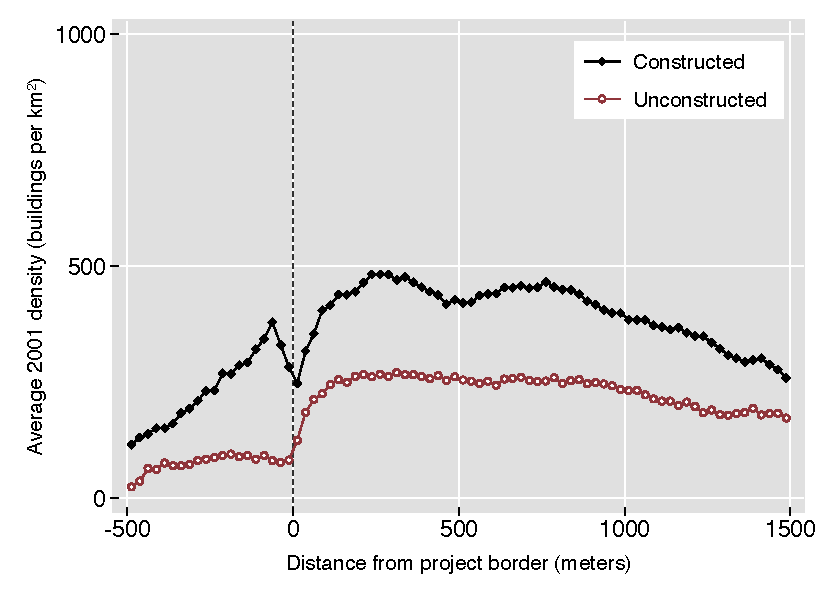
\includegraphics[width=\textwidth,trim={0.3cm .3cm 0.1cm 0cm}, clip=true]{figures/bblu_for_pre_means_4_spk.pdf}

        \end{subfigure}
        \hfill
        \begin{subfigure}[b]{0.48\textwidth}  
                    \caption[]%
            {{\footnotesize \textbf{All Projects} pre-period informal  raw data}}      
            \label{fig:preinf}
            \centering 
            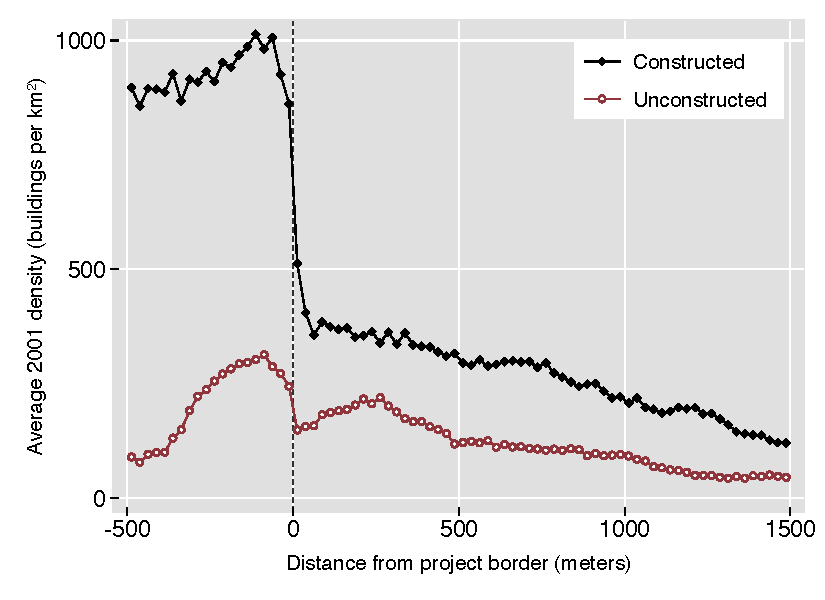
\includegraphics[width=\textwidth,trim={0.3cm .3cm 0.1cm 0cm}, clip=true]{figures/bblu_inf_pre_means_4_spk.pdf}

        \end{subfigure}
        \begin{subfigure}[b]{0.48\textwidth}
                    \caption[Network2]%
            {{\footnotesize \textbf{Greenfield} pre-period formal  raw data}}    
            \label{fig:prefor}
            \centering
            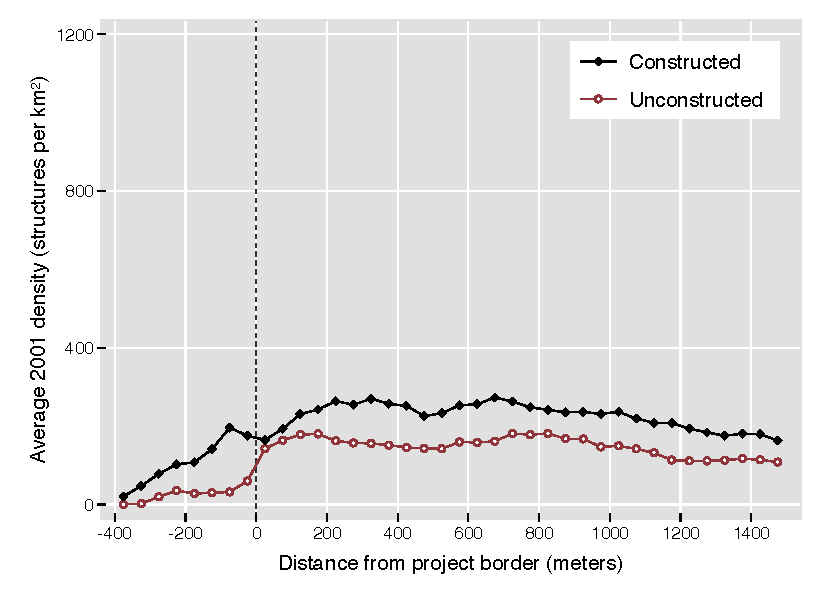
\includegraphics[width=\textwidth,trim={0.3cm .3cm 0.1cm 0cm}, clip=true]{figures/bblu_for_pre_means_4_1_spk.pdf}

        \end{subfigure}
        \hfill
        \begin{subfigure}[b]{0.48\textwidth}  
                    \caption[]%
            {{\footnotesize \textbf{Greenfield} pre-period informal  raw data}}     
            \label{fig:preinf}
            \centering 
            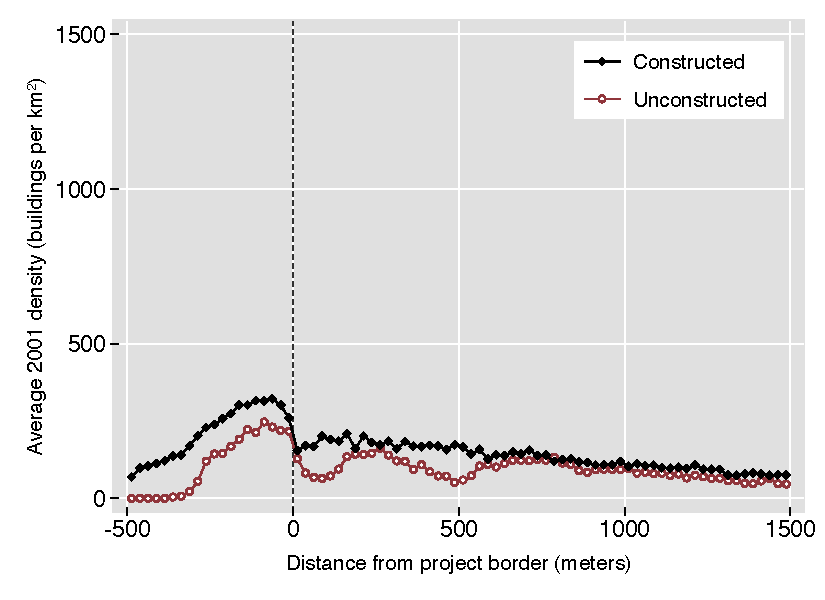
\includegraphics[width=\textwidth,trim={0.3cm .3cm 0.1cm 0cm}, clip=true]{figures/bblu_inf_pre_means_4_1_spk.pdf}

        \end{subfigure}
        \begin{subfigure}[b]{0.48\textwidth}
                    \caption[Network2]%
            {{\footnotesize \textbf{In-Situ} pre-period formal  raw data}}   
            \label{fig:prefor}
            \centering
            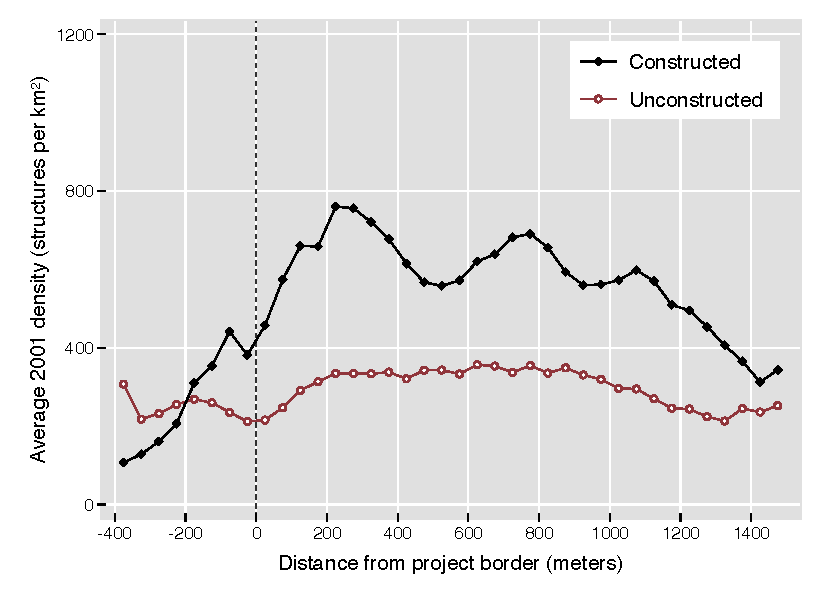
\includegraphics[width=\textwidth,trim={0.3cm .3cm 0.1cm 0cm}, clip=true]{figures/bblu_for_pre_means_4_2_spk.pdf}

        \end{subfigure}
        \hfill
        \begin{subfigure}[b]{0.48\textwidth}  
                    \caption[]%
            {{\footnotesize \textbf{In-Situ} pre-period informal  raw data}}     
            \label{fig:preinf}
            \centering 
            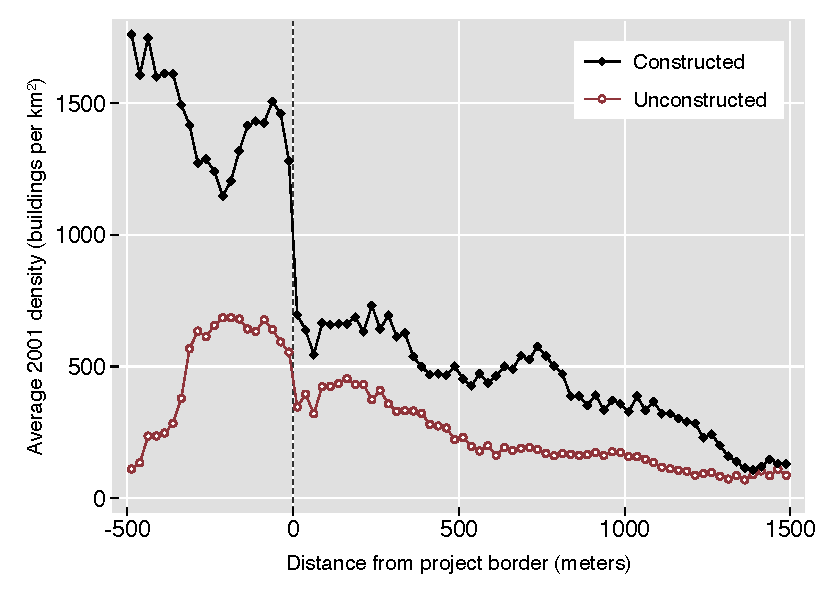
\includegraphics[width=\textwidth,trim={0.3cm .3cm 0.1cm 0cm}, clip=true]{figures/bblu_inf_pre_means_4_2_spk.pdf}

        \end{subfigure}
        \begin{subfigure}[b]{0.48\textwidth}
                    \caption[Network2]%
            {{\footnotesize \textbf{Other} pre-period formal  raw data}}   
            \label{fig:prefor}
            \centering
            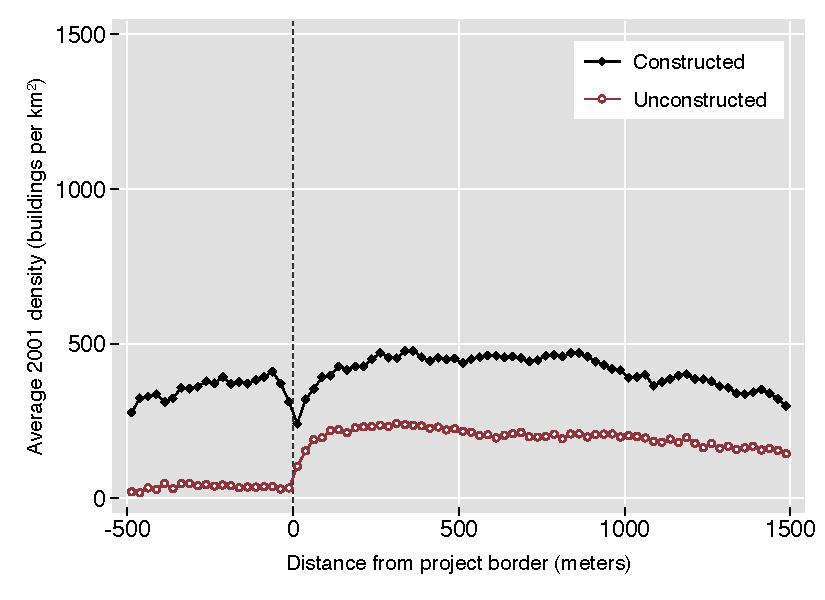
\includegraphics[width=\textwidth,trim={0.3cm .3cm 0.1cm 0cm}, clip=true]{figures/bblu_for_pre_means_4_3_spk.pdf}

        \end{subfigure}
        \hfill
        \begin{subfigure}[b]{0.48\textwidth}  
                    \caption[]%
            {{\footnotesize \textbf{Other} pre-period informal  raw data}}      
            \label{fig:preinf}
            \centering 
            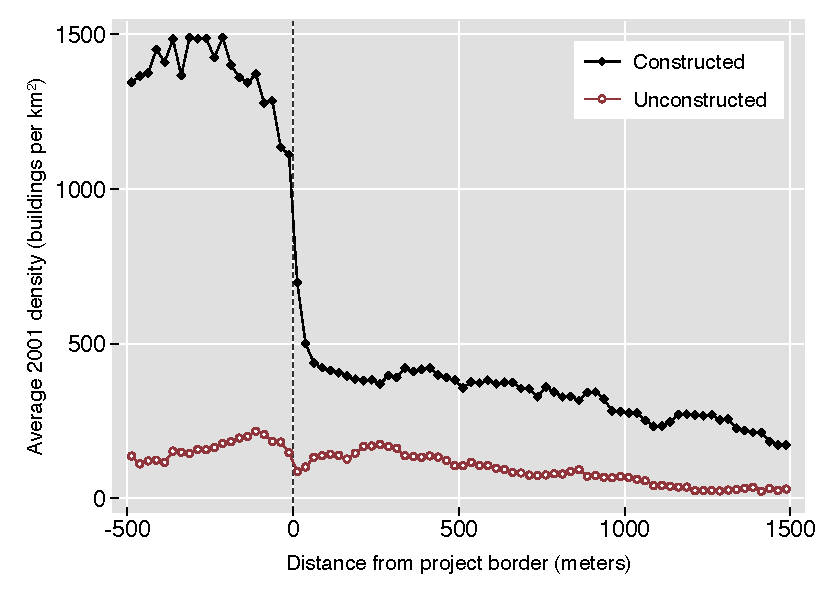
\includegraphics[width=\textwidth,trim={0.3cm .3cm 0.1cm 0cm}, clip=true]{figures/bblu_inf_pre_means_4_3_spk.pdf}

        \end{subfigure}
\end{figure*}


\begin{figure*}
        \centering
   %     \caption[ Pre-Period Housing Densities in Constructed and Unconstructed Projects Areas ]
  %      {\small Pre-Period Densities} 
        %\vspace{2mm}
        \begin{subfigure}[b]{0.48\textwidth}
                    \caption[Network2]%
            {{\footnotesize \textbf{All Projects} pre-period formal fe}}    
            \label{fig:prefor}
            \centering
            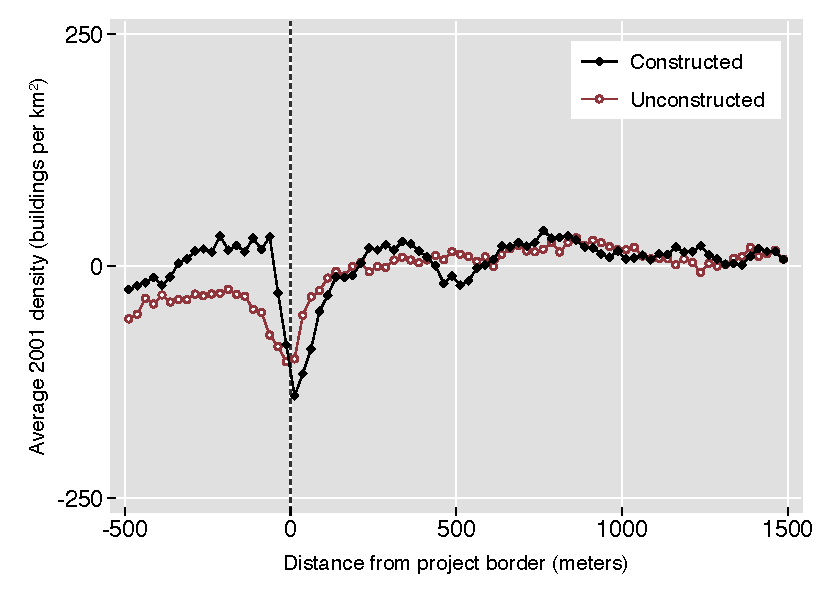
\includegraphics[width=\textwidth,trim={0.3cm .3cm 0.1cm 0cm}, clip=true]{figures/bblu_for_fe_pre_means_4_spk.pdf}

        \end{subfigure}
        \hfill
        \begin{subfigure}[b]{0.48\textwidth}  
                    \caption[]%
            {{\footnotesize \textbf{All Projects} pre-period informal fe }}      
            \label{fig:preinf}
            \centering 
            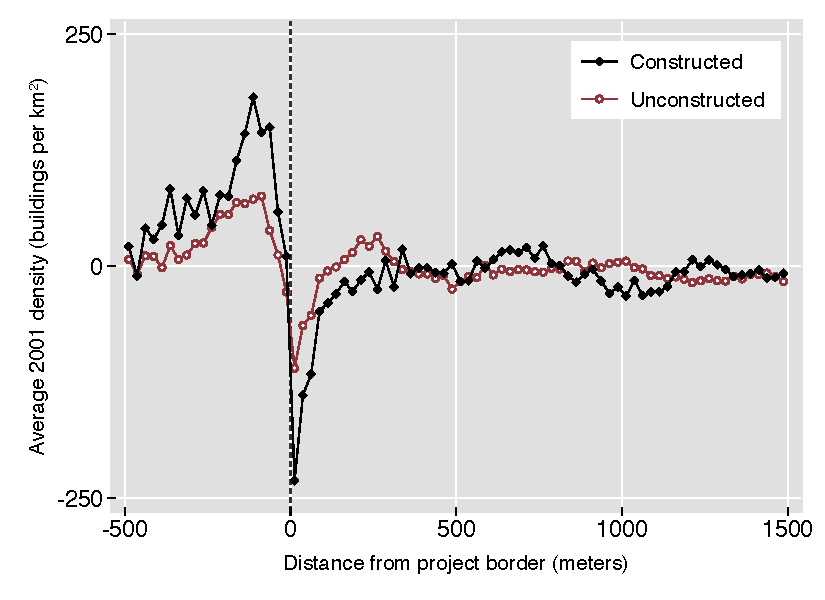
\includegraphics[width=\textwidth,trim={0.3cm .3cm 0.1cm 0cm}, clip=true]{figures/bblu_inf_fe_pre_means_4_spk.pdf}

        \end{subfigure}
        \begin{subfigure}[b]{0.48\textwidth}
                    \caption[Network2]%
            {{\footnotesize \textbf{Greenfield} pre-period formal  fe }}    
            \label{fig:prefor}
            \centering
            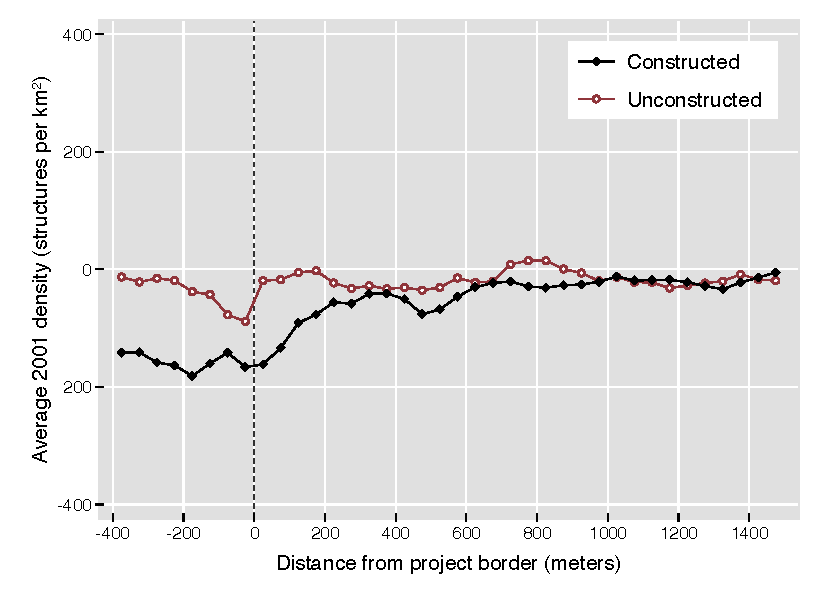
\includegraphics[width=\textwidth,trim={0.3cm .3cm 0.1cm 0cm}, clip=true]{figures/bblu_for_fe_pre_means_4_1_spk.pdf}

        \end{subfigure}
        \hfill
        \begin{subfigure}[b]{0.48\textwidth}  
                    \caption[]%
            {{\footnotesize \textbf{Greenfield} pre-period informal fe }}     
            \label{fig:preinf}
            \centering 
            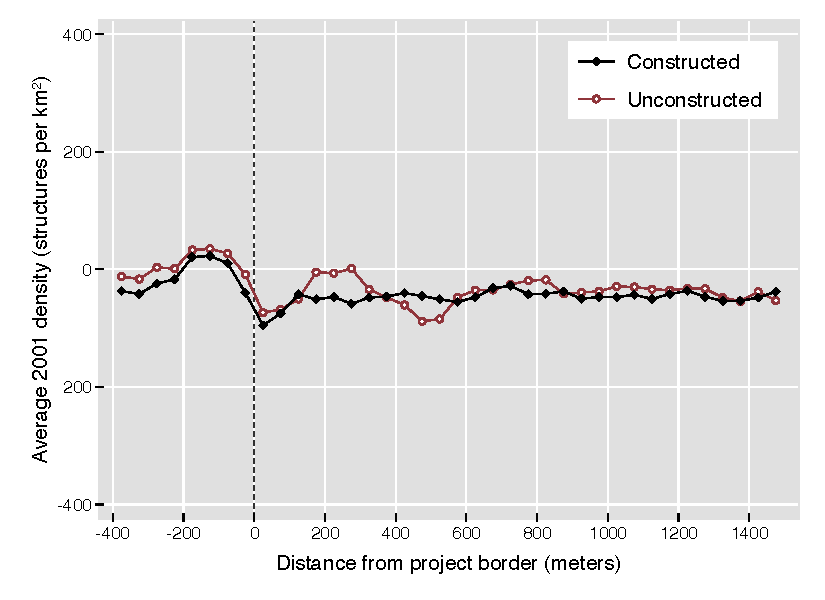
\includegraphics[width=\textwidth,trim={0.3cm .3cm 0.1cm 0cm}, clip=true]{figures/bblu_inf_fe_pre_means_4_1_spk.pdf}

        \end{subfigure}
        \begin{subfigure}[b]{0.48\textwidth}
                    \caption[Network2]%
            {{\footnotesize \textbf{In-Situ} pre-period formal fe }}   
            \label{fig:prefor}
            \centering
            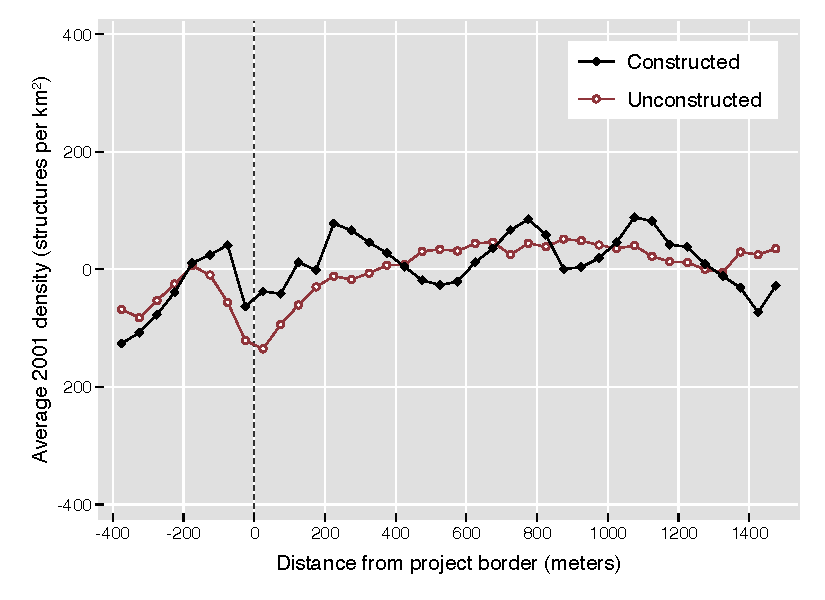
\includegraphics[width=\textwidth,trim={0.3cm .3cm 0.1cm 0cm}, clip=true]{figures/bblu_for_fe_pre_means_4_2_spk.pdf}

        \end{subfigure}
        \hfill
        \begin{subfigure}[b]{0.48\textwidth}  
                    \caption[]%
            {{\footnotesize \textbf{In-Situ} pre-period informal fe }}     
            \label{fig:preinf}
            \centering 
            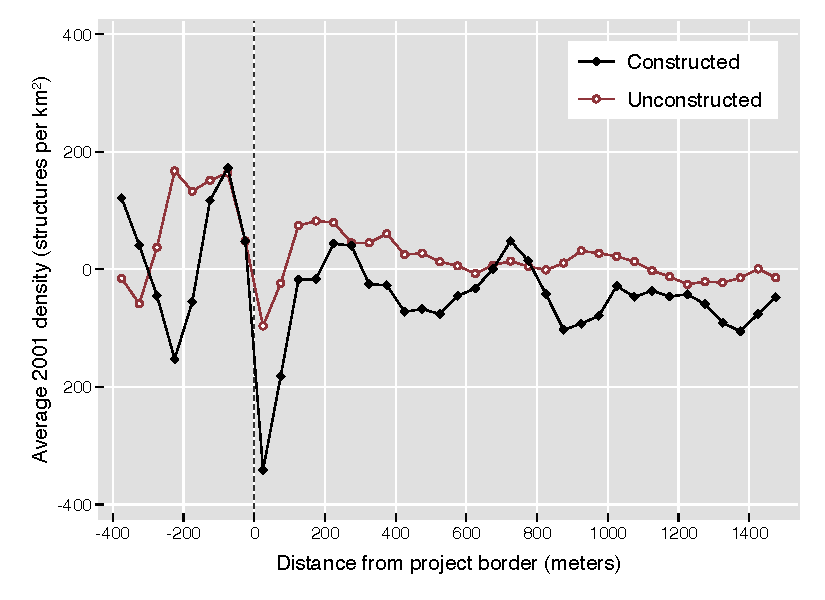
\includegraphics[width=\textwidth,trim={0.3cm .3cm 0.1cm 0cm}, clip=true]{figures/bblu_inf_fe_pre_means_4_2_spk.pdf}

        \end{subfigure}
        \begin{subfigure}[b]{0.48\textwidth}
                    \caption[Network2]%
            {{\footnotesize \textbf{Other} pre-period formal fe }}   
            \label{fig:prefor}
            \centering
            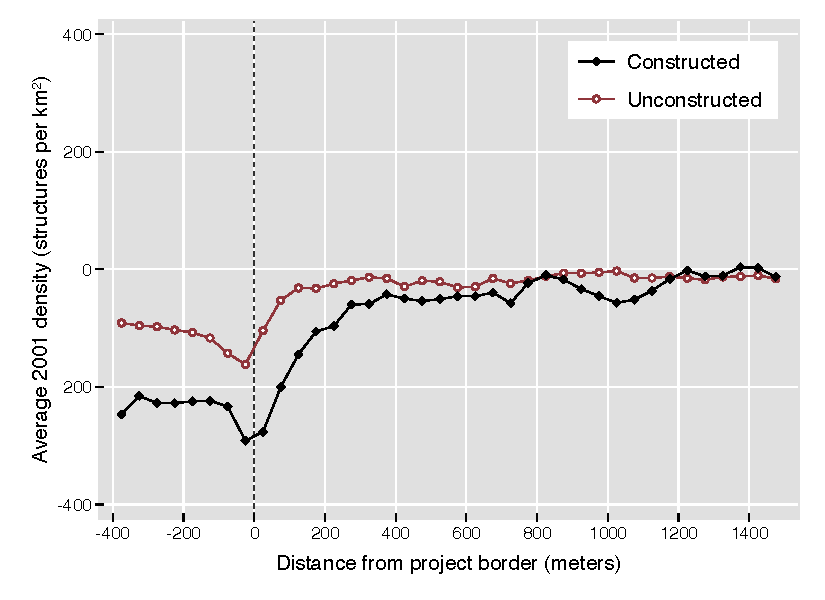
\includegraphics[width=\textwidth,trim={0.3cm .3cm 0.1cm 0cm}, clip=true]{figures/bblu_for_fe_pre_means_4_3_spk.pdf}

        \end{subfigure}
        \hfill
        \begin{subfigure}[b]{0.48\textwidth}  
                    \caption[]%
            {{\footnotesize \textbf{Other} pre-period informal fe }}      
            \label{fig:preinf}
            \centering 
            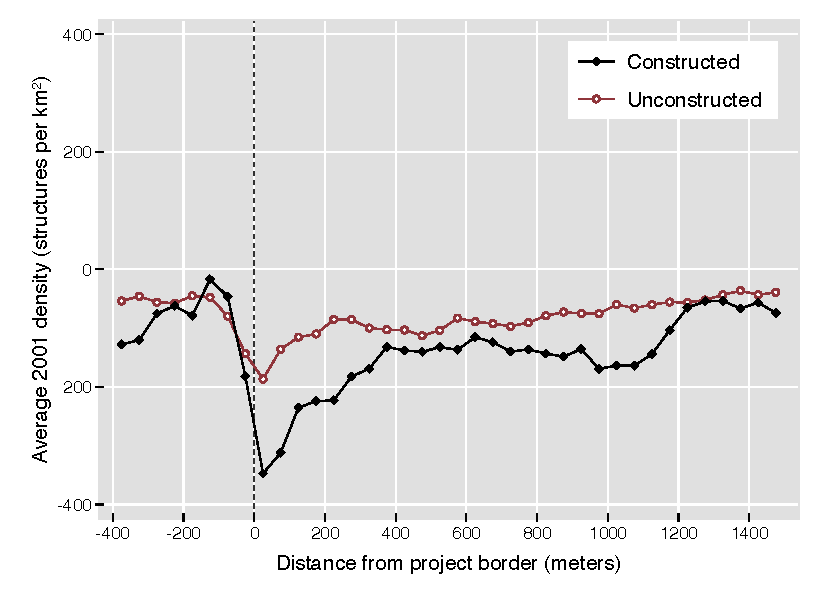
\includegraphics[width=\textwidth,trim={0.3cm .3cm 0.1cm 0cm}, clip=true]{figures/bblu_inf_fe_pre_means_4_3_spk.pdf}

        \end{subfigure}
\end{figure*}








\begin{figure*}
        \centering
   %     \caption[ Pre-Period Housing Densities in Constructed and Unconstructed Projects Areas ]
  %      {\small Pre-Period Densities} 
        %\vspace{2mm}
        \begin{subfigure}[b]{0.48\textwidth}
            \caption[Network2]%
            {{\footnotesize \textbf{All Projects} changes formal raw data}}    
            \label{fig:prefor}
            \centering
            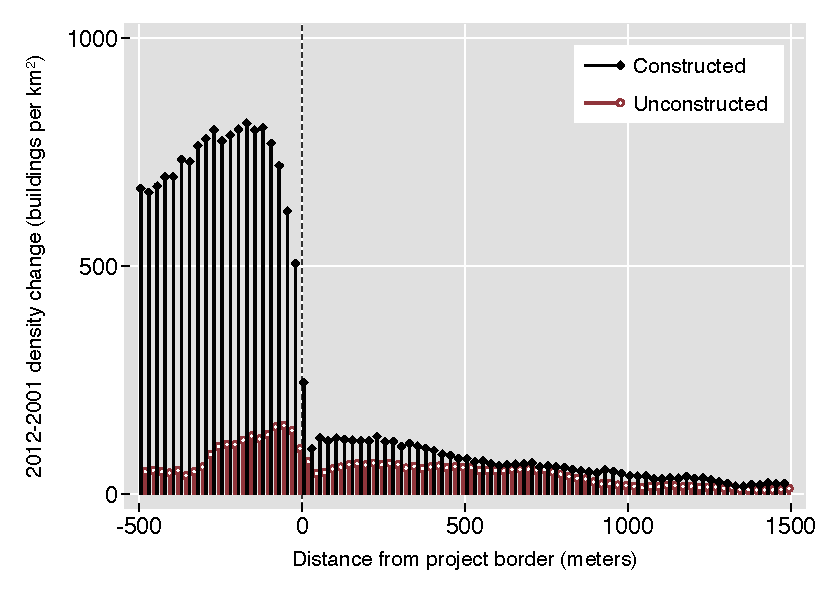
\includegraphics[width=\textwidth,trim={0.3cm .3cm 0.1cm 0cm}, clip=true]{figures/bblu_for_rawchanges_4_spk.pdf}

        \end{subfigure}
        \hfill
        \begin{subfigure}[b]{0.48\textwidth}  
                    \caption[]%
            {{\footnotesize \textbf{All Projects} changes informal  raw data}}      
            \label{fig:preinf}
            \centering 
            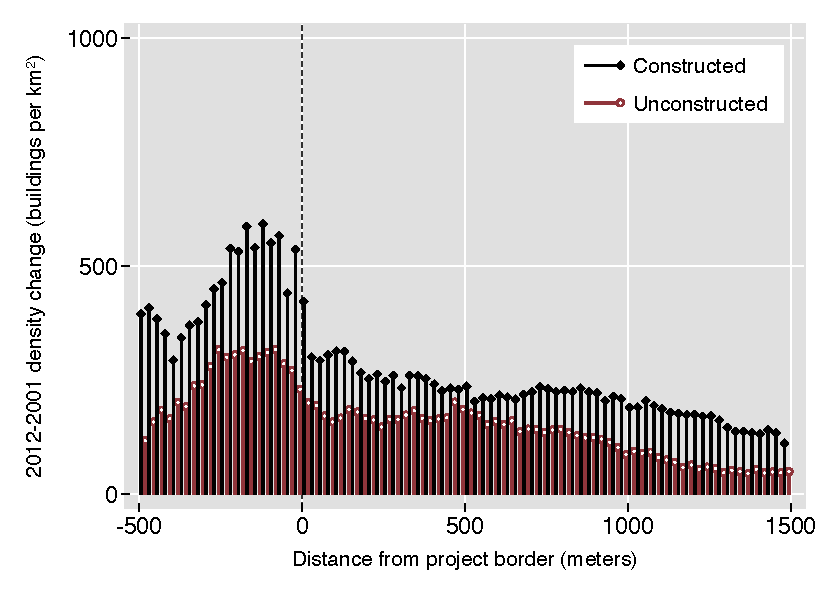
\includegraphics[width=\textwidth,trim={0.3cm .3cm 0.1cm 0cm}, clip=true]{figures/bblu_inf_rawchanges_4_spk.pdf}

        \end{subfigure}
        \begin{subfigure}[b]{0.48\textwidth}
                    \caption[Network2]%
            {{\footnotesize \textbf{Greenfield} changes formal  raw data}}    
            \label{fig:prefor}
            \centering
            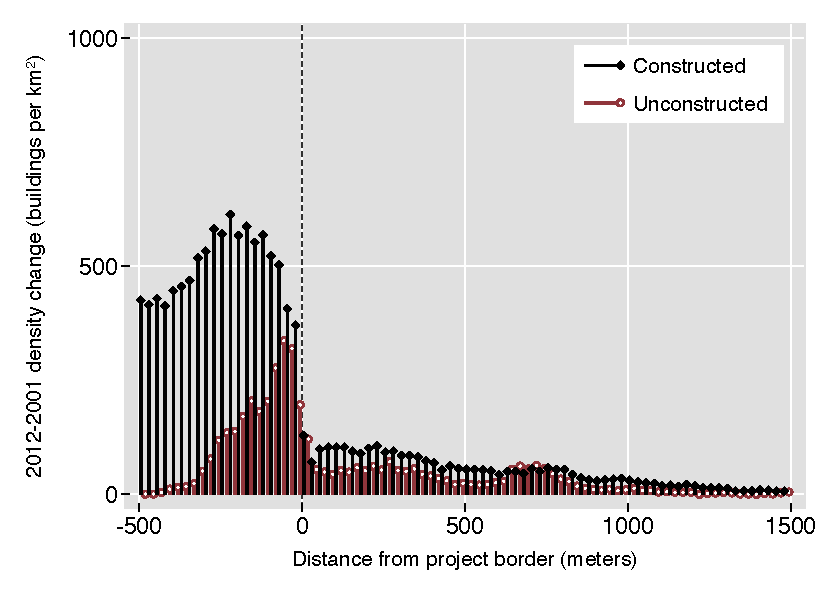
\includegraphics[width=\textwidth,trim={0.3cm .3cm 0.1cm 0cm}, clip=true]{figures/bblu_for_rawchanges_4_1_spk.pdf}

        \end{subfigure}
        \hfill
        \begin{subfigure}[b]{0.48\textwidth}  
                    \caption[]%
            {{\footnotesize \textbf{Greenfield} changes informal raw data }}     
            \label{fig:preinf}
            \centering 
            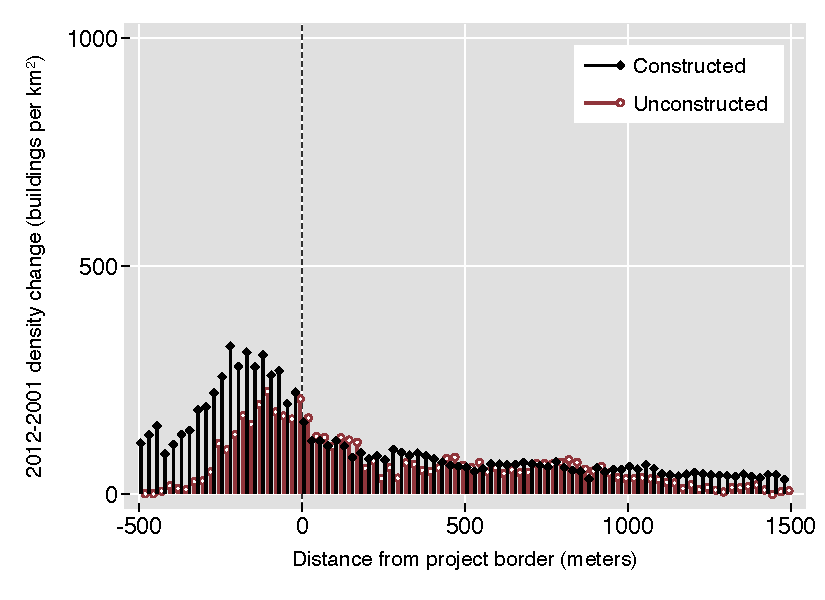
\includegraphics[width=\textwidth,trim={0.3cm .3cm 0.1cm 0cm}, clip=true]{figures/bblu_inf_rawchanges_4_1_spk.pdf}

        \end{subfigure}
        \begin{subfigure}[b]{0.48\textwidth}
                    \caption[Network2]%
            {{\footnotesize \textbf{In-Situ} changes formal raw data }}   
            \label{fig:prefor}
            \centering
            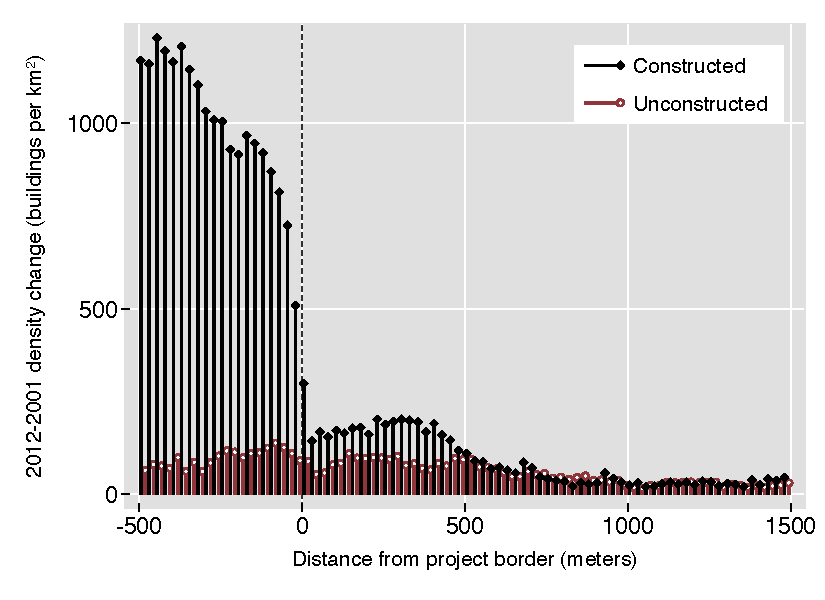
\includegraphics[width=\textwidth,trim={0.3cm .3cm 0.1cm 0cm}, clip=true]{figures/bblu_for_rawchanges_4_2_spk.pdf}

        \end{subfigure}
        \hfill
        \begin{subfigure}[b]{0.48\textwidth}  
                    \caption[]%
            {{\footnotesize \textbf{In-Situ} changes informal raw data }}     
            \label{fig:preinf}
            \centering 
            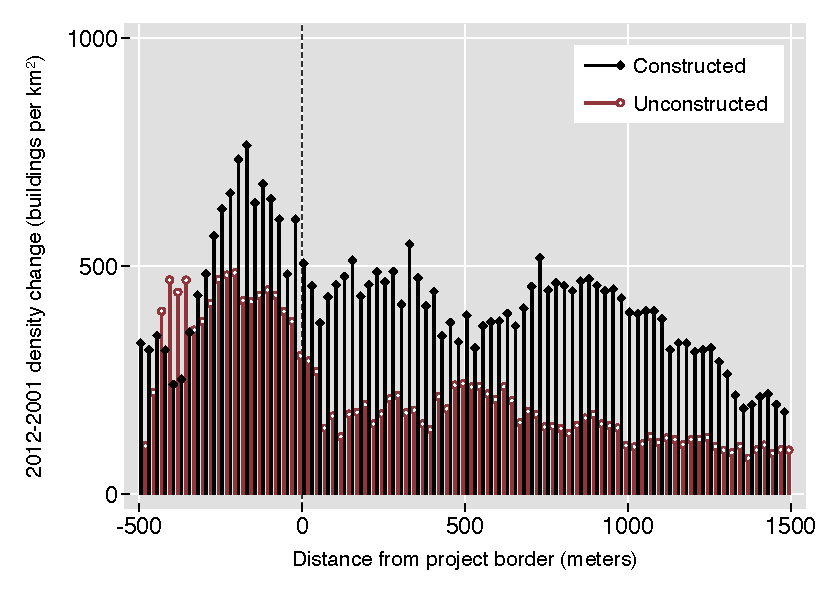
\includegraphics[width=\textwidth,trim={0.3cm .3cm 0.1cm 0cm}, clip=true]{figures/bblu_inf_rawchanges_4_2_spk.pdf}

        \end{subfigure}
        \begin{subfigure}[b]{0.48\textwidth}
                    \caption[Network2]%
            {{\footnotesize \textbf{Other} changes formal raw data}}   
            \label{fig:prefor}
            \centering
            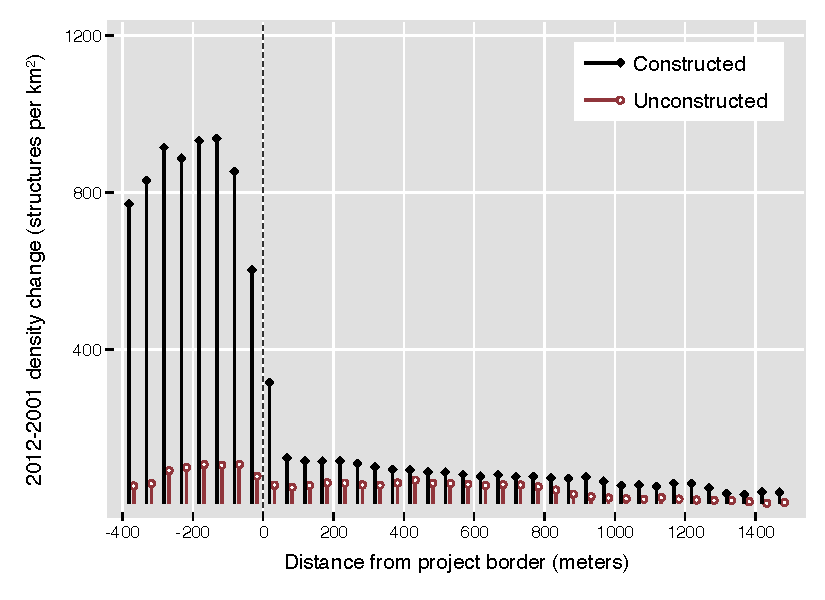
\includegraphics[width=\textwidth,trim={0.3cm .3cm 0.1cm 0cm}, clip=true]{figures/bblu_for_rawchanges_4_3_spk.pdf}

        \end{subfigure}
        \hfill
        \begin{subfigure}[b]{0.48\textwidth} 
                    \caption[]%
            {{\footnotesize \textbf{Other} changes informal  raw data}}      
            \label{fig:preinf} 
            \centering 
            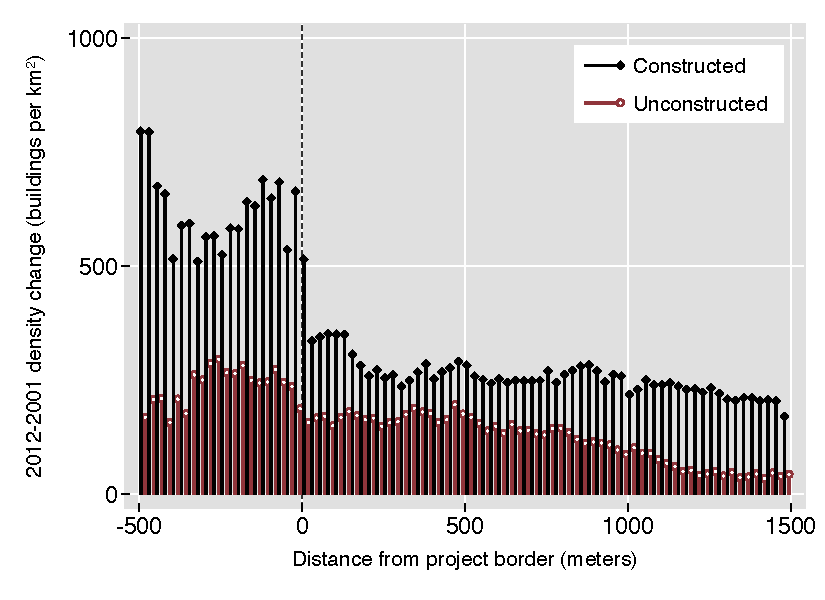
\includegraphics[width=\textwidth,trim={0.3cm .3cm 0.1cm 0cm}, clip=true]{figures/bblu_inf_rawchanges_4_3_spk.pdf}

        \end{subfigure}
\end{figure*}




\begin{figure*}
        \centering
   %     \caption[ Pre-Period Housing Densities in Constructed and Unconstructed Projects Areas ]
  %      {\small Pre-Period Densities} 
        %\vspace{2mm}
        \begin{subfigure}[b]{0.48\textwidth}
            \caption[Network2]%
            {{\footnotesize \textbf{All Projects} changes formal fe }}    
            \label{fig:prefor}
            \centering
            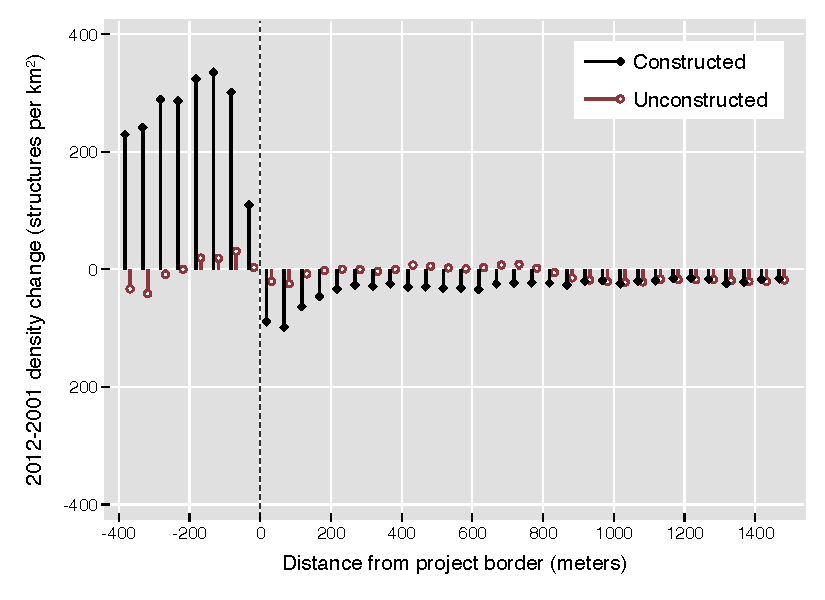
\includegraphics[width=\textwidth,trim={0.3cm .3cm 0.1cm 0cm}, clip=true]{figures/bblu_for_fe_rawchanges_4_spk.pdf}

        \end{subfigure}
        \hfill
        \begin{subfigure}[b]{0.48\textwidth}  
                    \caption[]%
            {{\footnotesize \textbf{All Projects} changes informal  fe }}      
            \label{fig:preinf}
            \centering 
            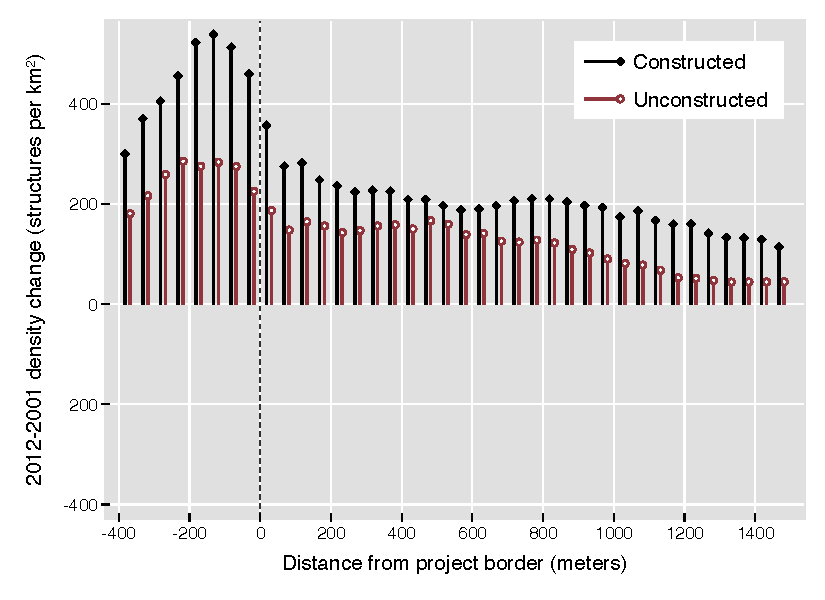
\includegraphics[width=\textwidth,trim={0.3cm .3cm 0.1cm 0cm}, clip=true]{figures/bblu_inf_fe_rawchanges_4_spk.pdf}

        \end{subfigure}
        \begin{subfigure}[b]{0.48\textwidth}
                    \caption[Network2]%
            {{\footnotesize \textbf{Greenfield} changes formal  fe}}    
            \label{fig:prefor}
            \centering
            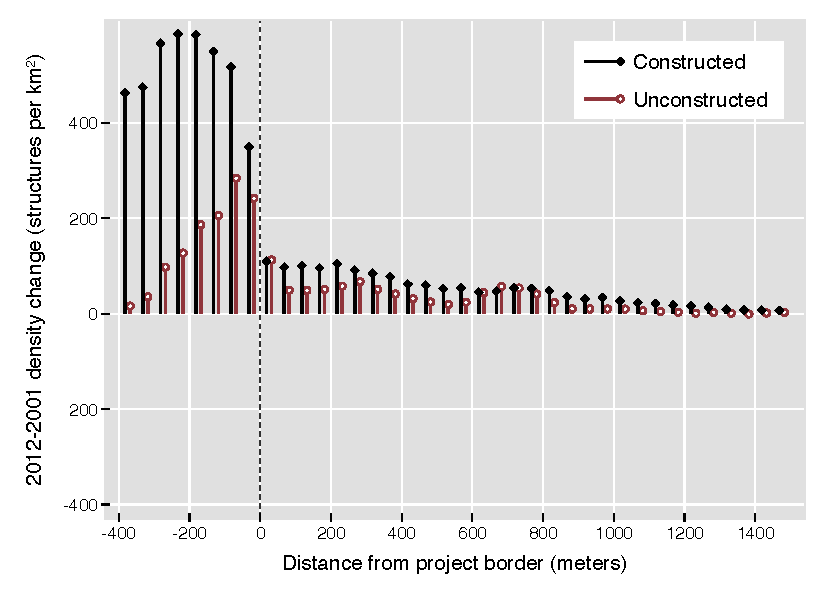
\includegraphics[width=\textwidth,trim={0.3cm .3cm 0.1cm 0cm}, clip=true]{figures/bblu_for_fe_rawchanges_4_1_spk.pdf}

        \end{subfigure}
        \hfill
        \begin{subfigure}[b]{0.48\textwidth}  
                    \caption[]%
            {{\footnotesize \textbf{Greenfield} changes informal fe}}     
            \label{fig:preinf}
            \centering 
            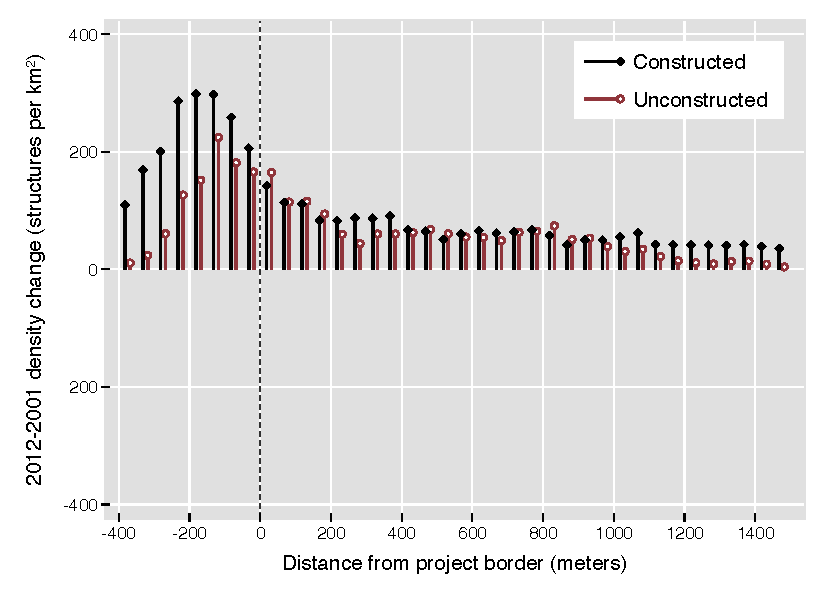
\includegraphics[width=\textwidth,trim={0.3cm .3cm 0.1cm 0cm}, clip=true]{figures/bblu_inf_fe_rawchanges_4_1_spk.pdf}

        \end{subfigure}
        \begin{subfigure}[b]{0.48\textwidth}
                    \caption[Network2]%
            {{\footnotesize \textbf{In-Situ} changes formal fe}}   
            \label{fig:prefor}
            \centering
            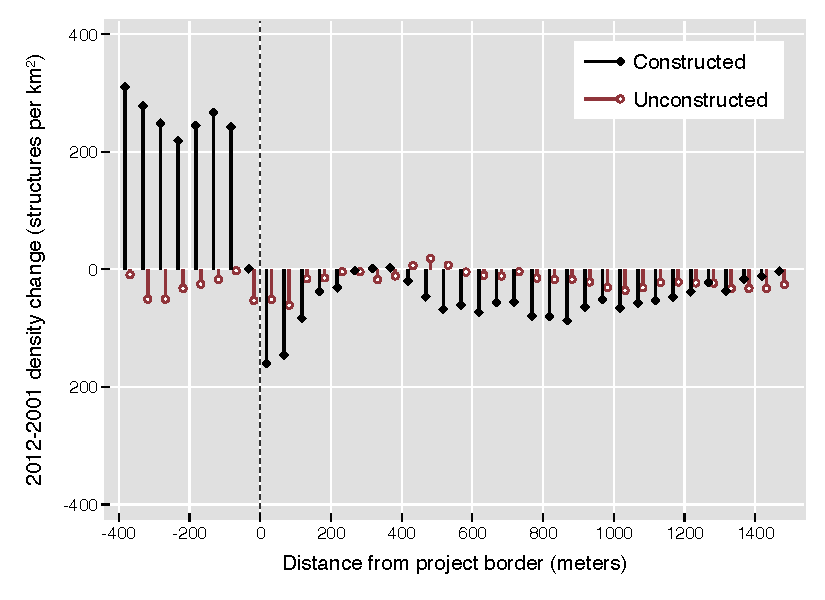
\includegraphics[width=\textwidth,trim={0.3cm .3cm 0.1cm 0cm}, clip=true]{figures/bblu_for_fe_rawchanges_4_2_spk.pdf}

        \end{subfigure}
        \hfill
        \begin{subfigure}[b]{0.48\textwidth}  
                    \caption[]%
            {{\footnotesize \textbf{In-Situ} changes informal fe}}     
            \label{fig:preinf}
            \centering 
            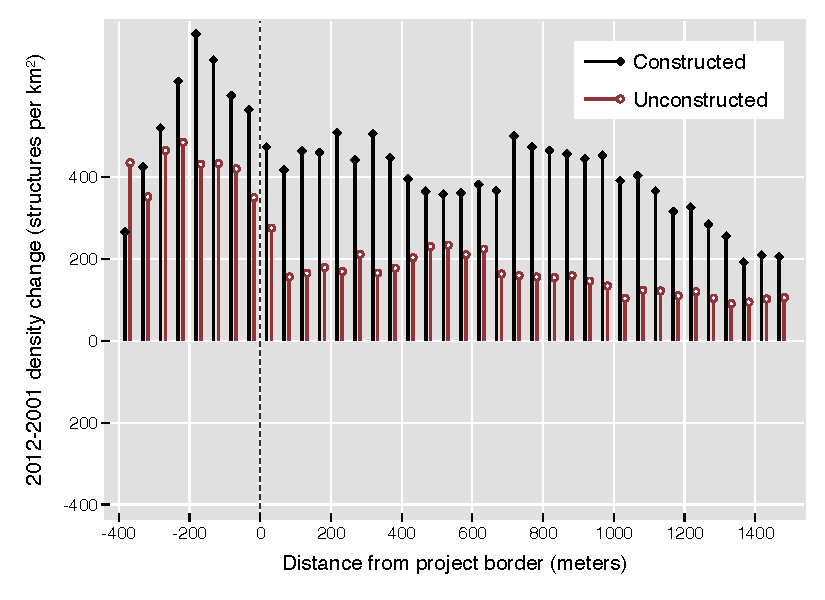
\includegraphics[width=\textwidth,trim={0.3cm .3cm 0.1cm 0cm}, clip=true]{figures/bblu_inf_fe_rawchanges_4_2_spk.pdf}

        \end{subfigure}
        \begin{subfigure}[b]{0.48\textwidth}
                    \caption[Network2]%
            {{\footnotesize \textbf{Other} changes formal fe}}   
            \label{fig:prefor}
            \centering
            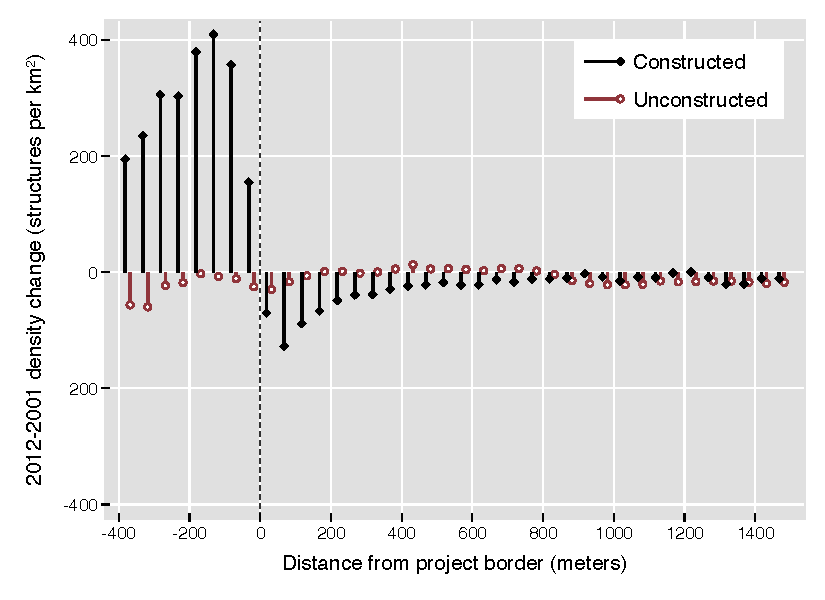
\includegraphics[width=\textwidth,trim={0.3cm .3cm 0.1cm 0cm}, clip=true]{figures/bblu_for_fe_rawchanges_4_3_spk.pdf}

        \end{subfigure}
        \hfill
        \begin{subfigure}[b]{0.48\textwidth} 
                    \caption[]%
            {{\footnotesize \textbf{Other} changes informal  fe}}      
            \label{fig:preinf} 
            \centering 
            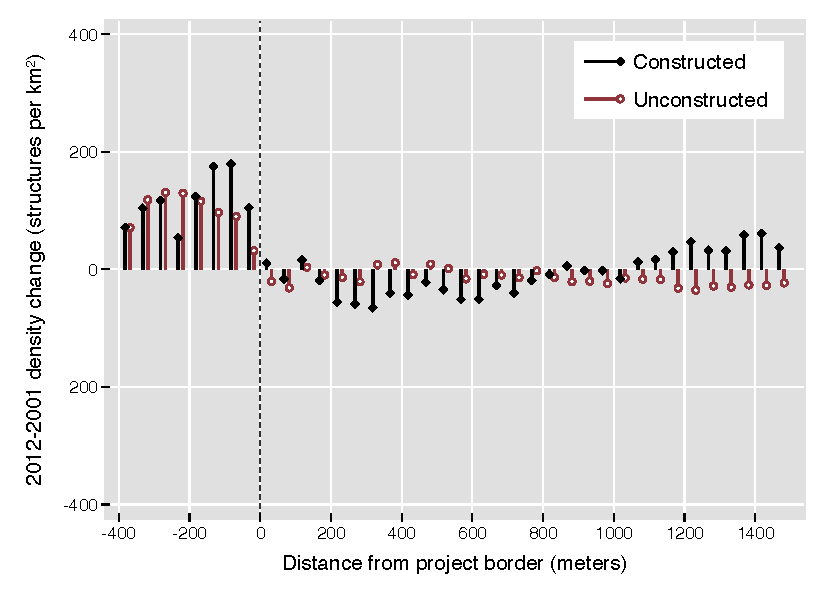
\includegraphics[width=\textwidth,trim={0.3cm .3cm 0.1cm 0cm}, clip=true]{figures/bblu_inf_fe_rawchanges_4_3_spk.pdf}

        \end{subfigure}
\end{figure*}







\begin{table}
\caption{Building Density}
\begin{tabular}{lDDDDD}
\toprule
 & \small (1) & \small (2)  & \small (3) & \small (4) & \small (5) \\
 & Total & Formal  & Informal & Informal Bkyd. & Informal Non-Bkyd. \\ \midrule
\textbf{All Projects} \\inside project      &     649.922\textsuperscript{a}&     578.443\textsuperscript{a}&      71.480                   &     504.849\textsuperscript{a}&    -433.370\textsuperscript{a}\\
                    &   (142.616)                   &    (74.820)                   &   (109.424)                   &   (103.825)                   &    (87.292)                   \\[0.5em]
0-300m outside project &      -4.615                   &      34.561                   &     -39.176                   &       6.232                   &     -45.408                   \\
                    &    (43.557)                   &    (24.468)                   &    (35.476)                   &    (31.666)                   &    (28.686)                   \\[0.5em]
300-600m outside project &     -93.284\textsuperscript{b}&      -4.618                   &     -88.666\textsuperscript{a}&     -65.122\textsuperscript{b}&     -23.544                   \\
                    &    (37.628)                   &    (16.270)                   &    (33.167)                   &    (28.288)                   &    (16.895)                   \\[0.5em]
R$^2$               &       0.448                   &       0.414                   &       0.398                   &       0.344                   &       0.337                   \\

\midrule
\textbf{Greenfield} \\   inside project      &     361.753                   &     306.915\textsuperscript{b}&      54.838                   &     127.892                   &     -73.054                   \\
                    &   (229.486)                   &   (147.158)                   &   (110.523)                   &   (121.834)                   &    (58.122)                   \\[0.01em]
0-300m outside project &     -53.158                   &     -12.367                   &     -40.791                   &     -63.823                   &      23.032                   \\
                    &    (95.533)                   &    (47.250)                   &    (63.258)                   &    (60.774)                   &    (47.707)                   \\[0.01em]
300-600m outside project&     -49.582                   &      -9.003                   &     -40.579                   &     -32.918                   &      -7.661                   \\
                    &    (51.568)                   &    (23.797)                   &    (32.897)                   &    (21.415)                   &    (19.889)                   \\[0.8em] 
\textbf{In-Situ Upgrading} \\   inside project      &     565.065                   &     809.800\textsuperscript{a}&    -244.736                   &     658.644\textsuperscript{b}&    -903.380\textsuperscript{a}\\
                    &   (356.225)                   &   (142.934)                   &   (276.805)                   &   (267.350)                   &   (234.007)                   \\[0.01em]
0-300m outside project &      48.642                   &      88.579                   &     -39.937                   &      29.298                   &     -69.236                   \\
                    &   (143.656)                   &    (88.007)                   &   (109.649)                   &   (128.896)                   &    (95.077)                   \\[0.01em]
300-600m outside project &     -18.405                   &      64.735                   &     -83.140                   &     -73.815                   &      -9.325                   \\
                    &    (99.320)                   &    (59.952)                   &    (85.012)                   &    (89.071)                   &    (69.369)                   \\[0.8em]
\textbf{Other} \\   inside project      &     872.541\textsuperscript{a}&     662.918\textsuperscript{a}&     209.623                   &     665.246\textsuperscript{a}&    -455.623\textsuperscript{a}\\
                    &   (179.383)                   &    (76.252)                   &   (147.435)                   &   (117.301)                   &   (102.382)                   \\[0.01em]
0-300m outside project &     -11.076                   &      36.434                   &     -47.511                   &       8.864                   &     -56.374                   \\
                    &    (69.233)                   &    (27.094)                   &    (58.467)                   &    (43.920)                   &    (38.256)                   \\[0.01em]
300-600m outside project &    -130.682\textsuperscript{b}&     -21.257                   &    -109.425\textsuperscript{b}&     -67.915\textsuperscript{c}&     -41.510\textsuperscript{b}\\
                    &    (50.317)                   &    (18.695)                   &    (45.840)                   &    (39.079)                   &    (20.527)                   \\[0.8em]
Mean Outcome 2001   &      379.90                   &      203.91                   &      175.98                   &       66.26                   &      109.72                   \\
Mean Outcome 2011   &      584.70                   &      281.66                   &      303.04                   &      192.77                   &      110.27                   \\
R$^2$               &       0.451                   &       0.416                   &       0.401                   &       0.351                   &       0.339                   \\
N                   &   2,721,910                   &   2,721,910                   &   2,721,910                   &   2,721,910                   &   2,721,910                   \\

\bottomrule
\end{tabular}
\end{table}





\begin{table}[h!] 
\caption{Effect of Housing Projects on Socio-demographics}
\label{table:sorting}
\small
\centering
%\caption{Census Composition Estimates }
\vspace{-2mm}
\begin{tabular}{lDDDDD}
\toprule
& \small (1) & \small (2) & \small (3) & \small (4)& \small (5)\\
& \small Age & \small P.O.B. not Gauteng & \small Unemployed & \small Years of Education & \small Monthly Income \\ \midrule 
\textbf{All Projects} \\inside project      &      -0.100                   &      -0.011                   &       0.019                   &       0.223\textsuperscript{c}&    1287.718\textsuperscript{b}\\
                    &     (0.291)                   &     (0.019)                   &     (0.019)                   &     (0.124)                   &   (509.978)                   \\[0.5em]
0-300m outside project &       0.445\textsuperscript{c}&      -0.013                   &       0.007                   &       0.087                   &     639.143                   \\
                    &     (0.258)                   &     (0.015)                   &     (0.017)                   &     (0.100)                   &   (502.951)                   \\[0.5em]
300-600m outside project &      -0.290                   &       0.005                   &       0.010                   &      -0.041                   &     124.114                   \\
                    &     (0.308)                   &     (0.015)                   &     (0.015)                   &     (0.102)                   &   (456.986)                   \\[0.5em]
R$^2$               &       0.630                   &       0.743                   &       0.480                   &       0.659                   &       0.605                   \\

\midrule
\textbf{Greenfield} \\   inside project      &      -0.954                   &      -0.013                   &       0.063                   &      -0.056                   &     922.823                   \\
                    &     (0.606)                   &     (0.058)                   &     (0.039)                   &     (0.254)                   &   (693.091)                   \\[0.01em]
0-300m outside project &      -0.065                   &      -0.002                   &       0.041                   &      -0.099                   &     165.112                   \\
                    &     (0.617)                   &     (0.029)                   &     (0.047)                   &     (0.218)                   &   (698.387)                   \\[0.01em]
300-600m outside project&      -0.853                   &       0.011                   &       0.024                   &       0.427\textsuperscript{c}&     172.723                   \\
                    &     (0.591)                   &     (0.039)                   &     (0.031)                   &     (0.238)                   &   (528.057)                   \\[0.8em] 
\textbf{In-Situ Upgrading} \\   inside project      &       0.352                   &       0.011                   &      -0.008                   &       0.190                   &     451.113                   \\
                    &     (0.377)                   &     (0.018)                   &     (0.034)                   &     (0.198)                   &   (904.739)                   \\[0.01em]
0-300m outside project &       0.143                   &      -0.018                   &       0.000                   &       0.208                   &     537.741                   \\
                    &     (0.336)                   &     (0.019)                   &     (0.031)                   &     (0.186)                   &   (959.019)                   \\[0.01em]
300-600m outside project &      -1.091                   &       0.023                   &       0.003                   &      -0.240                   &   -1028.250                   \\
                    &     (0.690)                   &     (0.023)                   &     (0.029)                   &     (0.204)                   &   (943.118)                   \\[0.8em]
\textbf{Other} \\   inside project      &      -0.032                   &      -0.023                   &       0.024                   &       0.252                   &    2014.760\textsuperscript{a}\\
                    &     (0.444)                   &     (0.025)                   &     (0.025)                   &     (0.180)                   &   (604.348)                   \\[0.01em]
0-300m outside project &       0.802\textsuperscript{b}&      -0.012                   &      -0.004                   &       0.057                   &    1037.459\textsuperscript{c}\\
                    &     (0.369)                   &     (0.020)                   &     (0.024)                   &     (0.140)                   &   (588.483)                   \\[0.01em]
300-600m outside project &       0.302                   &      -0.007                   &       0.002                   &      -0.091                   &     873.321                   \\
                    &     (0.408)                   &     (0.019)                   &     (0.020)                   &     (0.148)                   &   (620.709)                   \\[0.8em]
Mean Outcome 2001   &       27.30                   &        0.37                   &        0.47                   &        8.26                   &    2,475.96                   \\
Mean Outcome 2011   &       28.30                   &        0.43                   &        0.33                   &        9.68                   &    4,486.48                   \\
R$^2$               &       0.633                   &       0.745                   &       0.482                   &       0.661                   &       0.610                   \\
N                   &      12,733                   &      12,726                   &      12,723                   &      12,727                   &      12,723                   \\

\bottomrule
\multicolumn{6}{l}{\footnotesize Standard errors clustered at the project level in parenthesis. \textsuperscript{c} p$<$0.10, \textsuperscript{b} p$<$0.05, \textsuperscript{a} p$<$0.01  }\\
\multicolumn{6}{l}{\footnotesize P.O.B. means ``place of birth.''  Monthly income is in Rands.}
\end{tabular}
\end{table}








\begin{landscape}
{\footnotesize

\begin{table}[]
\small
\centering
\caption{Census Household-level Estimates }\label{table:censusestimates}
\vspace{-2mm}
\resizebox{.9\linewidth}{!}{
\begin{tabular}{lDDDDDDDD}
\toprule
 & \small (1) & \small (2)  & \small (3) & \small (4) & \small (5)  & \small (6)  & \small (7) & (8)\\
 & \small Flush Toilet & \small Water Indoors  & \small Electricity Cooking & \small Electricity Heating & \small Electricity Lighting  & \small Number of Rooms  & \small Household Size & Population Density\\ \midrule 
\textbf{All Projects} \\inside project      &       0.117                   &       0.131\textsuperscript{a}&       0.174\textsuperscript{b}&       0.110                   &       0.061                   &       0.159                   &       0.110                   &   -1140.587                   \\
                    &     (0.077)                   &     (0.036)                   &     (0.073)                   &     (0.067)                   &     (0.077)                   &     (0.150)                   &     (0.094)                   &  (1314.840)                   \\[0.5em]
0-300m outside project &       0.021                   &       0.037                   &       0.056                   &       0.040                   &       0.030                   &       0.191                   &       0.052                   &   -1171.220                   \\
                    &     (0.034)                   &     (0.038)                   &     (0.036)                   &     (0.041)                   &     (0.032)                   &     (0.118)                   &     (0.059)                   &   (786.833)                   \\[0.5em]
300-600m outside project &      -0.001                   &       0.030                   &       0.021                   &       0.023                   &      -0.007                   &       0.012                   &       0.030                   &   -1447.534                   \\
                    &     (0.022)                   &     (0.032)                   &     (0.026)                   &     (0.031)                   &     (0.024)                   &     (0.110)                   &     (0.058)                   &  (1262.516)                   \\[0.5em]
R$^2$               &       0.530                   &       0.541                   &       0.584                   &       0.549                   &       0.556                   &       0.631                   &       0.632                   &       0.561                   \\

\midrule
\textbf{Greenfield} \\   inside project      &       0.126                   &       0.128                   &       0.172                   &       0.093                   &       0.154                   &       0.409                   &       0.203                   &    3352.649                   \\
                    &     (0.110)                   &     (0.109)                   &     (0.117)                   &     (0.131)                   &     (0.103)                   &     (0.290)                   &     (0.199)                   &  (2646.595)                   \\[0.01em]
0-300m outside project &      -0.055                   &       0.028                   &      -0.042                   &      -0.036                   &      -0.001                   &       0.195                   &       0.340\textsuperscript{b}&     289.860                   \\
                    &     (0.060)                   &     (0.095)                   &     (0.073)                   &     (0.080)                   &     (0.056)                   &     (0.285)                   &     (0.151)                   &  (1470.092)                   \\[0.01em]
300-600m outside project&       0.022                   &       0.077                   &       0.025                   &       0.015                   &       0.065                   &       0.267                   &       0.157                   &   -4985.461                   \\
                    &     (0.057)                   &     (0.086)                   &     (0.055)                   &     (0.064)                   &     (0.044)                   &     (0.297)                   &     (0.162)                   &  (4988.849)                   \\[0.8em] 
\textbf{In-Situ Upgrading} \\   inside project      &       0.316\textsuperscript{b}&       0.134\textsuperscript{c}&       0.161                   &       0.144                   &       0.056                   &       0.168                   &       0.099                   &   -4454.400                   \\
                    &     (0.151)                   &     (0.069)                   &     (0.105)                   &     (0.093)                   &     (0.100)                   &     (0.213)                   &     (0.153)                   &  (3025.393)                   \\[0.01em]
0-300m outside project &       0.036                   &      -0.008                   &       0.058                   &       0.034                   &       0.040                   &      -0.183                   &      -0.036                   &   -1647.754                   \\
                    &     (0.075)                   &     (0.084)                   &     (0.071)                   &     (0.088)                   &     (0.065)                   &     (0.240)                   &     (0.089)                   &  (1551.069)                   \\[0.01em]
300-600m outside project &       0.000                   &       0.012                   &       0.068                   &       0.109                   &      -0.012                   &      -0.186                   &      -0.030                   &      11.233                   \\
                    &     (0.049)                   &     (0.062)                   &     (0.057)                   &     (0.073)                   &     (0.059)                   &     (0.256)                   &     (0.092)                   &  (1445.302)                   \\[0.8em]
\textbf{Other} \\   inside project      &      -0.024                   &       0.151\textsuperscript{a}&       0.158                   &       0.089                   &       0.030                   &       0.051                   &       0.052                   &    -602.172                   \\
                    &     (0.103)                   &     (0.047)                   &     (0.113)                   &     (0.104)                   &     (0.122)                   &     (0.234)                   &     (0.126)                   &   (995.680)                   \\[0.01em]
0-300m outside project &       0.021                   &       0.075                   &       0.052                   &       0.044                   &       0.014                   &       0.394\textsuperscript{a}&      -0.004                   &   -1782.150\textsuperscript{c}\\
                    &     (0.043)                   &     (0.047)                   &     (0.045)                   &     (0.047)                   &     (0.041)                   &     (0.152)                   &     (0.068)                   &   (981.425)                   \\[0.01em]
300-600m outside project &      -0.001                   &       0.046                   &       0.016                   &       0.010                   &      -0.015                   &       0.089                   &      -0.002                   &   -1683.528\textsuperscript{c}\\
                    &     (0.031)                   &     (0.045)                   &     (0.027)                   &     (0.030)                   &     (0.026)                   &     (0.136)                   &     (0.066)                   &   (901.989)                   \\[0.8em]
Mean Outcome 2001   &        0.79                   &        0.35                   &        0.66                   &        0.62                   &        0.77                   &        3.30                   &        3.51                   &    8,566.83                   \\
Mean Outcome 2011   &        0.83                   &        0.54                   &        0.81                   &        0.72                   &        0.82                   &        3.56                   &        3.18                   &    9,823.82                   \\
R$^2$               &       0.543                   &       0.552                   &       0.592                   &       0.558                   &       0.564                   &       0.636                   &       0.635                   &       0.564                   \\
N                   &      12,732                   &      12,732                   &      12,732                   &      12,732                   &      12,732                   &      12,709                   &      12,730                   &      12,734                   \\

\bottomrule
\multicolumn{9}{l}{\footnotesize All regressions include 3km grid Fixed-Effects. Standard errors clustered at the project level in parenthesis. \textsuperscript{c} p$<$0.10,\textsuperscript{b} p$<$0.05,\textsuperscript{a} p$<$0.01 }
\end{tabular}
}
\end{table}

}
\end{landscape}




\begin{table}
\small
\centering
\caption{Triple Difference Estimates on Log-Prices}\label{table:priceDDD_het}
\vspace{-2mm}
\begin{tabular}{lCC}
\toprule
 & \small (1) & \small (2)  \\ \midrule 
 \textbf{All Projects} \\
 inside project      &      -0.206                   &      -0.183                   \\
                    &     (0.256)                   &     (0.252)                   \\[0.55em]
0-300m outside project &      -0.112\textsuperscript{c}&      -0.107                   \\
                    &     (0.066)                   &     (0.066)                   \\[0.5em]
300-600m outside project &      -0.065                   &      -0.066                   \\
                    &     (0.054)                   &     (0.054)                   \\[0.5em]
Lot Size Controls   &                               &  \checkmark                   \\
r2                  &        0.45                   &        0.45                   \\
N                   &      67,751                   &      67,751                   \\

 \midrule
\textbf{Greenfield} \\   inside project      &       0.165                   &       0.107                   \\
                    &     (0.174)                   &     (0.164)                   \\[0.01em]
0-300m outside project &       0.080                   &       0.084                   \\
                    &     (0.151)                   &     (0.150)                   \\[0.01em]
300-600m outside project&      -0.037                   &      -0.039                   \\
                    &     (0.128)                   &     (0.129)                   \\[0.8em]
\textbf{In-Situ Upgrading} \\   inside project      &       0.368\textsuperscript{c}&       0.440\textsuperscript{b}\\
                    &     (0.205)                   &     (0.220)                   \\[0.01em]
0-300m outside project &      -0.301\textsuperscript{a}&      -0.302\textsuperscript{a}\\
                    &     (0.113)                   &     (0.112)                   \\[0.01em]
300-600m outside project &      -0.132                   &      -0.136                   \\
                    &     (0.099)                   &     (0.100)                   \\[0.8em]
\textbf{Other} \\   inside project      &      -0.415                   &      -0.377                   \\
                    &     (0.319)                   &     (0.312)                   \\[0.01em]
0-300m outside project &      -0.026                   &      -0.020                   \\
                    &     (0.091)                   &     (0.091)                   \\[0.01em]
300-600m outside project &      -0.054                   &      -0.054                   \\
                    &     (0.080)                   &     (0.081)                   \\[0.8em]
Lot Size Controls   &                               &  \checkmark                   \\
r2                  &        0.45                   &        0.46                   \\
N                   &      67,751                   &      67,751                   \\

\bottomrule
\multicolumn{3}{l}{\footnotesize Standard errors clustered at the project level in parenthesis.} \\
\multicolumn{3}{l}{ \textsuperscript{c} p$<$0.10,\textsuperscript{b} p$<$0.05,\textsuperscript{a} p$<$0.01 }
\end{tabular}
\end{table} 

% \begin{figure}
% 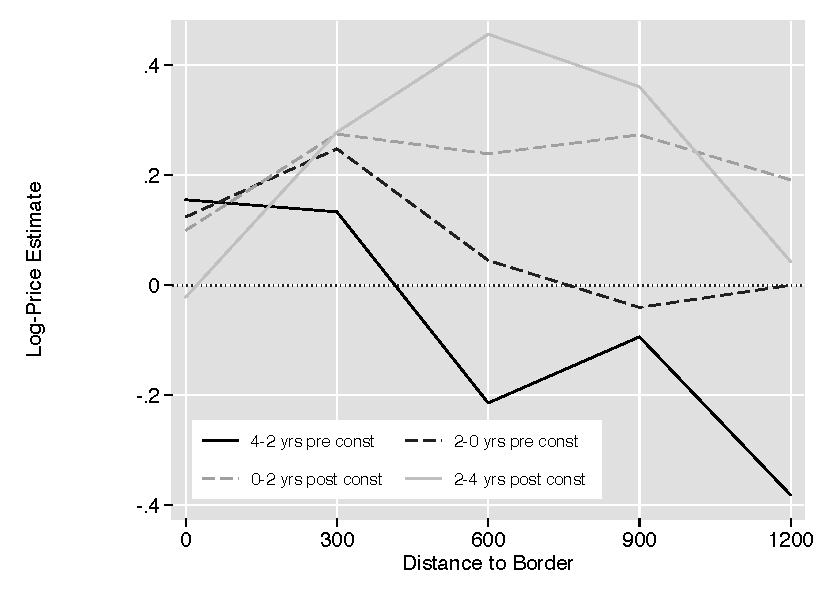
\includegraphics{figures/price_to_event_30.pdf}
% \end{figure}


\end{document}


